\documentclass{beamer}
\usetheme{default}
\begin{document}
%--------------------------------------------------

\begin{frame}
\begin{Huge}
\begin{center}
\textrm{UNIX \& Comandos basicos}
\end{center}

\end{Huge}
\end{frame}

%--------------------------------------------------


\begin{frame}{\textsc{UNIX}}

{\LARGE \textrm{Unix es un sistema operativo dise\~nado en los a\~nos 60's con el fin de ofrecer estabilidad en ambientes multi-usuario y multi-tarea.}}

\end{frame}

%--------------------------------------------------


\begin{frame}{\textrm{UNIX}}

\textrm{SO mas usado en el mundo:}
\begin{figure}
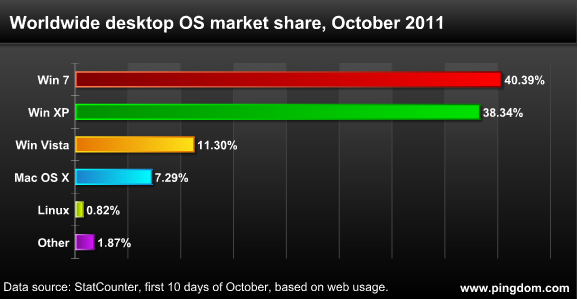
\includegraphics[scale=0.25]{fig2.png}
\end{figure}
{\scriptsize \textrm{Tomado de: http://www.pingdom.com}}\\
\textrm{SO mas usado por astronomos:}
\begin{figure}
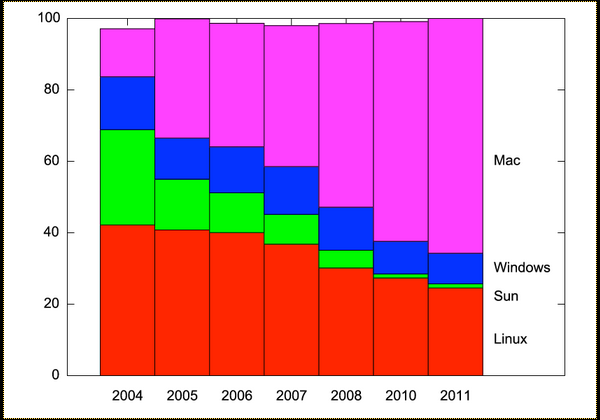
\includegraphics[scale=0.2]{fig1.png}
\end{figure}
{\scriptsize \textrm{Tomado de: http://www.astrobetter.com/os-apt-astronomers/}}\\


\end{frame}

%--------------------------------------------------


\begin{frame}{\textsc{Como empezar a usar UNIX?}}

\begin{Large}
\textrm{La Terminal es el lugar en el cual se controla la maquina.
All\'i se escibre texto el cual es interpretado por la maquina como comandos.}
\end{Large}

\begin{figure}
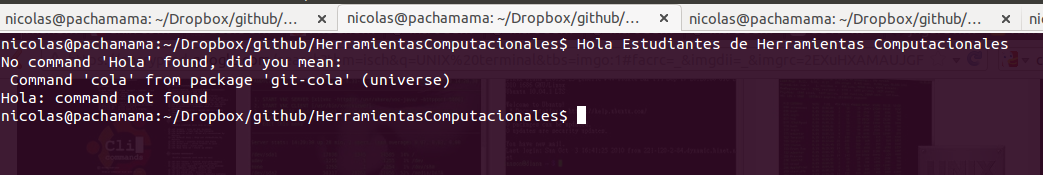
\includegraphics[scale=0.3]{fig3.png}
\end{figure}

\end{frame}

%--------------------------------------------------


\begin{frame}{\textsc{Comandos basicos:}}

\begin{center}
{\large \textsc{Directorios:}}
\end{center}
\begin{itemize}
\item \texttt{pwd}: \textrm{En que directorio estoy.}\\
\item \texttt{ls}: \textrm{Muestra los directorios que hay.}\\
\item \texttt{mkdir directorio}: \textrm{Crea un directorio llamado \texttt{directorio}}. 
\item \texttt{rmdir directorio}: \textrm{Elimina el directorio llamado \texttt{directorio}}.
\end{itemize}

\end{frame}


%--------------------------------------------------


\begin{frame}{\textsc{Comandos basicos:}}

\begin{center}
{\large \textsc{Archivos:}}
\end{center}

\begin{itemize}
\item \texttt{mv archivo1 archivo2:} \textrm{Mueve} \texttt{archivo1} \textrm{a} \texttt{archivo2}.
\item \texttt{cp:archivo1 archivo2} \textrm{Copia} \texttt{archivo1} \textrm{a} \texttt{archivo2}.
\item \texttt{rm archivo:} \textrm{Borra} \texttt{archivo}.
\item \texttt{less archivo:} \textrm{Permite ver dentro de} \texttt{archivo.}
\item \texttt{head archivo:} \textrm{Muestra las primeras 10 lin\'eas de} \texttt{archivo.}
\item \texttt{tail arhcivo:} \textrm{Muestra las ultimas 10 lin\'eas de} \texttt{archivo}.
\item \texttt{cat archivo1 archivo2:} \textrm{Concatena} \texttt:{archivo1} \textrm{con} \texttt{archivo2}.
\item \texttt{grep 'palabra' archivo:} \textrm{busca} \texttt{palabra} \textrm{dentro de} \texttt{archivo}.
\item \texttt{wc archivo:} \textrm{Imprime numero de lineas, palabras y bytes en} \texttt{archivo.}
\end{itemize}
\end{frame}

%--------------------------------------------------


\begin{frame}{\textsc{Comandos basicos:}}

\begin{center}
{\large \textsc{Comandos utiles:}}
\end{center}

\begin{itemize}
\item \texttt{man command:} \textrm{Muestra el manual de} \texttt{command}.
\item \texttt{history:} \textrm{Muestra una lista de los ultimos comandos utilizados.}
\item \texttt{Ctrl-r:} \textrm{Busca en la historia de comandos.}
\item \textrm{Tab:} \textrm{Presionar Tab en la mitad de un comando o un archivo y se mostraran opciones para completarlo.}
\end{itemize}

\end{frame}

%--------------------------------------------------

\begin{frame}{\textsc{hands-on}}

\begin{center}
{\Large \textrm{ir a: }}\\

https://github.com/jngaravitoc/HerramientasComputacionales.
\end{center}

\end{frame}

%----------------------------------------------------

\end{document}